%\section{Risk management approach \label{sect:approach}}

\subsection{Domains of risk}
See also the definitions section of \citell{LPM-20}.

In the general context of project management, a risk is defined as a threat to project success because it has a negative impact on cost, schedule or technical performance. 

As the primary products of DM are scientific in nature, any threat that could reduce or limit the scientific performance of the data processing can be considered as a risk. This includes factors that may have a  negative impact on the precision of the data processing results. It is worth noting in this context that computing performance of the implemented SW systems can have an indirect impact on scientific performance, as implemented SW must be able to process a certain volume of data in a limited amount of time. Assuming that SW has been efficiently implemented, this constraint can place limits on the algorithms that can be adopted; if the computational cost of an algorithm is too large a less accurate (but faster) algorithm would be preferred. Therefore, if something might increase the computational cost of the data processing (i.e. an increase in the number of objects to be processed, or an increase in algorithmic complexity to reach a desired scientific precision, etc.), it represents a risk to the scientific performance.

\subsection{Risk validity/Identification}

A valid DM risk impacts one or more of the three domains: resources, schedule or performance (see previous section).

One of the first tasks of the risk management process is to consider and discuss proposed risks, determine their validity and select those risks which are to be documented (see task one in section \ref{sect:strategy}).

Here are some examples of proposed risks  and the outcome expected from such a discussion.

\subsubsection*{Proposed risk 1:}

Real data is far more complex and quite different to the simulated data. Processing especially Alerts production is more computationally intensive and complex.
Practically all missions experience this.	

Expected conclusion:\\
Not accepted to be recorded as a risk because the proposal itself points out that real data will be more complex, so it is normal work to design, develop and plan for it.	

\subsubsection*{Proposed risk 2:}

Calculations made by  one group indicate that the hardware for the computationally intensive tasks it needs to perform does not scale well. Delay may occur while the technical solution is investigated.	
	
Expected conclusion:\\
This risk could be easily recorded with related severity and likelihood criteria. The initial actions and mitigation processes would be put into place,  for example: \\
a)	look for alternative hardware solutions (may increase cost, but could recover schedule)\\
b)	set a firm date for the first technical assessment and call a DMLT meeting to address alternative and solutions.	

The first example above is intended to illustrate a poor or bad risk proposal and the second is an example of a likely and reasonable proposal.

In general, a properly identified risk is composed of both cause and consequence, \citell{LPM-20} identifies the following list of assessment criteria:
\begin{enumerate}
\item {\bf Identification : } 
identifying elements of risk or opportunity in the subsystem or Project.
\item {\bf Establishing  time  frame :}
    determining  the  likely  time at  which a  risk or  opportunity event would come to pass.
\item {\bf Assessing  probability :  }
  estimating  the  probability  that  an  undesirable (for  risks)  or desirable (for opportunities) event may occur.
\item {\bf Assessing  severity :} 
   gauging  the  severity  of  the  impact  that  such  an  event  would  have on the status of the project if the event were to occur.  
\item {\bf Developing risk /opportunity handling options :}   
\begin{itemize}
\item  For  risks: developing  plans to  avoid, accept, mitigate, or transfer
\item  For opportunities: developing plans to permit or promote
\end{itemize}

\item {\bf Developing  a  management  response : }
 consider  how  the  project  may  respond  if  the event should occur
\end{enumerate}

In addition for DM we should determine if the risk merits promotion to the project level risk register. 

\subsection{Risk scoring: severity and likelihood \label{sect:scoring}}

Risk scoring is an attempt to qualitatively assess risks, and thus serves as an aid to objectively decide whether a risk merits attention, i.e. whether preemptive action should be taken to address the risk. Typically the two most important qualities of a risk that determines its seriousness is {\em severity} and {\em likelihood}.

For DM risk management, we adopt the severity and likelihood scales detailed below.

Risk severity is an evaluation of the consequences should a risk occur, and is measured using the following scale:
{\color{red} Not exactly what happens in LSST .. we may need to look at this}

\begin{tabular}{|l|l|p{0.75\linewidth}|} \hline
Score & Severity & Consequences of occurrence \\ \hline
5 & Catastrophic & Impact on resources, schedule and/or performance leads to the termination of the project. \\ \hline
4 & Critical & Final data production is compromised, either by significantly degrading its final quality so that several mission requirements will not be met,
and/or delaying its release by more than a year. Delay in first light  is required. Major resource re-allocation or acquisition perhaps at the telescope. \\ \hline
3 & Major & Occurrence causes a delay in the delivery of a non schedule critical component of more than one cycle, impacting the schedule of more than one part of DM over more than one cycle. Resources must be re-allocated between group or additional funds required, requiring intervention of LSST Project Manager. Final products are potentially compromised, so that one or more requirements will not be met unless new methods are developed or new resources can be found. \\ \hline
2 & Significant & Occurrence implies the delivery of a low quality product (component/algorithm/data is sub-optimal, not up to specs, incomplete, etc.) on time, or a delay is necessary to reach spec. Re-assignment of resources are necessary, but adjustments can be made within the group. Schedule of more than one part of DM is compromised, but original schedule can be re-attained after 1 cycle (some development cycle milestones must be postponed to next cycle, but no more). Final products may be compromised, but all mission requirements are met. \\ \hline
1 & Negligible & Occurrence implies some slight degradation in the quality of delivered product. Schedule of current cycle stressed, even compromised, but no impact on subsequent cycles. \\ \hline
\end{tabular}

Note: If any one of the consequences of a given severity applies, then the risk is at that specified severity level.
Also note: Severity is determined according to consequences to the DM as a whole.

Risk likelihood is an estimate of how likely the risk may actually happen. \figref{fig:lh} shows the scale from \citell{LPM-20}

\begin{figure}
\begin{center}
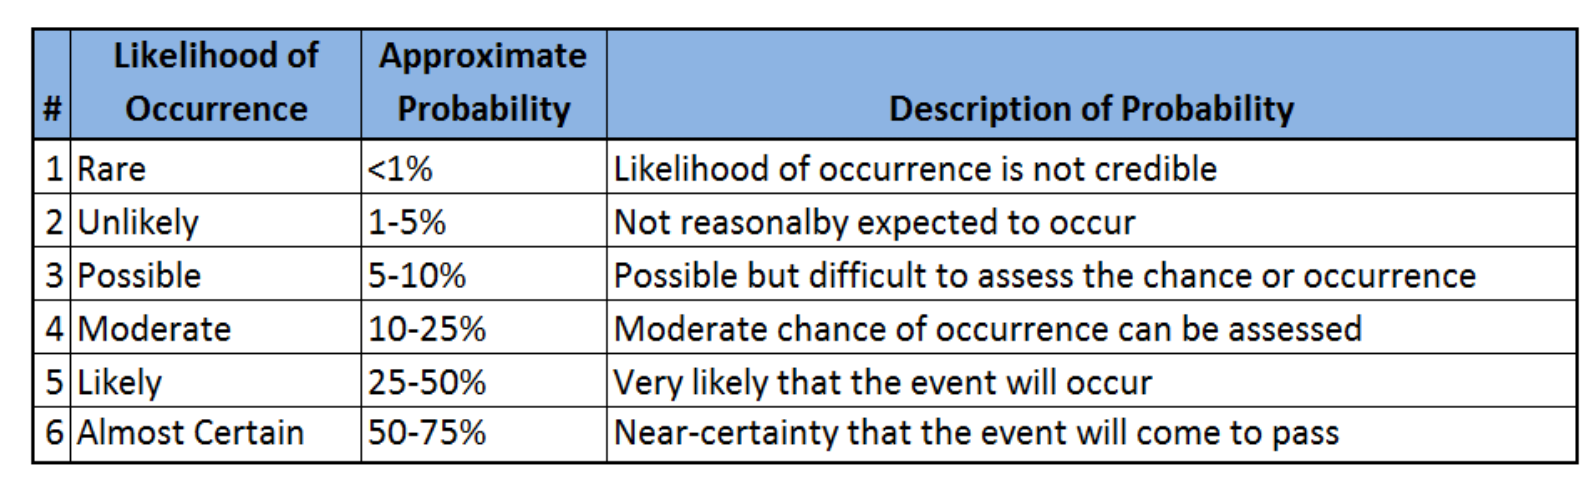
\includegraphics[width=0.8\textwidth]{images/lh}
\caption{Likelihood scale for risks from \citell{LPM-20}.\label{fig:lh}}
\end{center}

\end{figure}

These two scales (for severity and likelihood) define a two-dimensional space on which a given risk may be quantitatively mapped and thus assessed. A single code that describes the risk assessment can be constructed from these two scales, for example an A1 risk is a risk with minimum likelihood and minimum severity, while an E2 risk is a risk with significant impact that will certainly happen at least once in the next development cycles.

An acceptance regime (used to decide whether to accept a risk or take action to reduce the risk) is defined in the severity-likelihood plane in the next section \ref{sect:acceptance}.

It may be useful to reduce the two measures above to a single {\em risk index}, for the purpose of prioritising a list of risks or monitoring risks over time. An example of a risk index is shown in figure \ref{fig:riskindex}, showing a rating going from "Very Low" to "Very High".

  \begin{figure}[H]
  \begin{center}
  	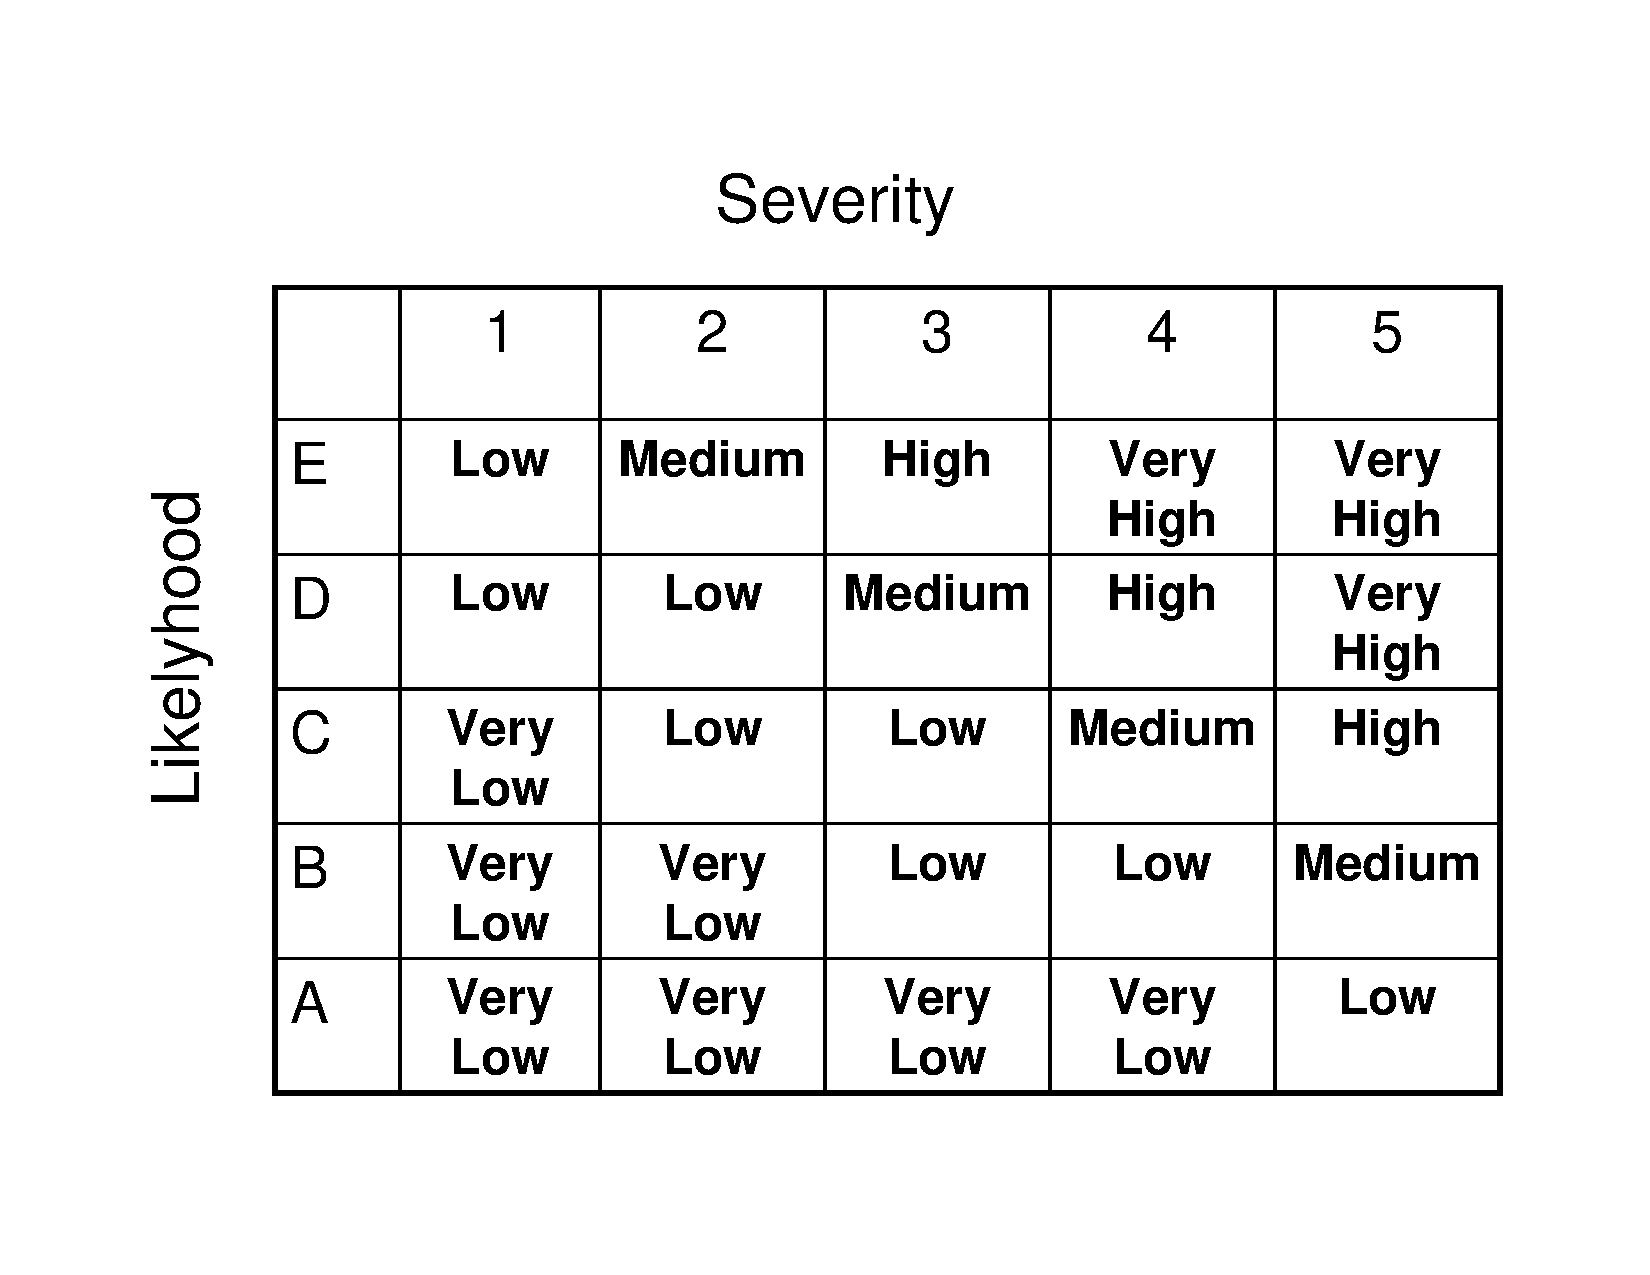
\includegraphics[scale=0.5]{images/RiskIndex}
  \end{center}
\vspace{-2cm}
\caption{Risk Index \label{fig:riskindex}}
   \end{figure}

Finally, it is worth mentioning that while the above scores and indices are quantitative they are still subjective measures, and thus can only serve as aids in the risk management process. There is no substitutes for good judgement based on experience.

\subsection{Risk acceptance \label{sect:acceptance}}

The risk scores are used to define criteria for acceptance or an acceptance regime in the severity-likelihood plane. This acceptance regime is shown in figure \ref{fig:regime}.

  \begin{figure}[H]
  \begin{center}
  	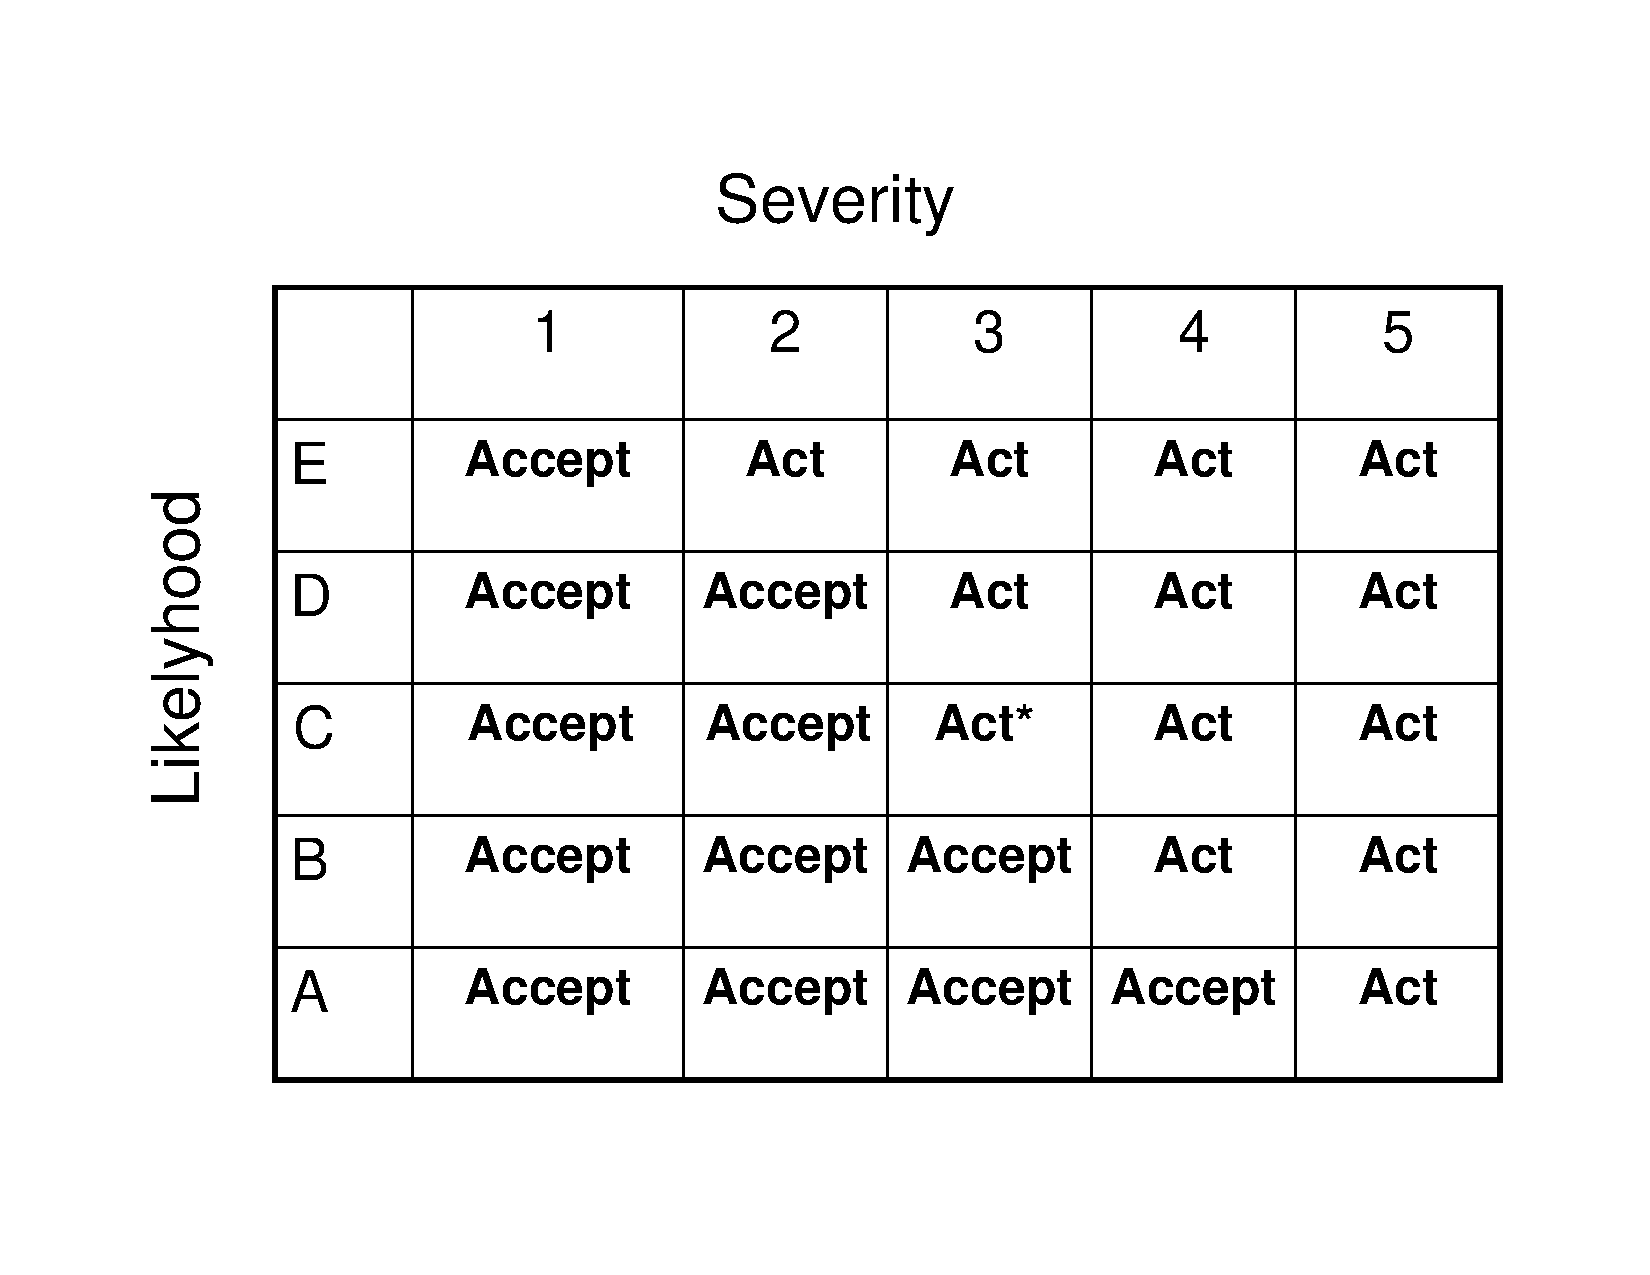
\includegraphics[scale=0.5]{images/AcceptanceRegime}
  \end{center}
\vspace{-2cm}
\caption{Acceptance regime \label{fig:regime}}
   \end{figure}

It should be noted that it is not required for a risk to fall in the acceptance regime for the RMT to recommend acceptance, particularly risks with a 'C' likelihood and a '3' severity criteria (see task 5 in section \ref{sect:strategy}).
